\documentclass[12pt]{article}
\usepackage[english]{babel}
\usepackage[utf8]{inputenc}

%% Pointer to 'default' preamble, other reusable files
% pacakages and definitions

\usepackage{geometry}
\geometry{
	letterpaper, 
	portrait, 
	top=.75in,
	left=.8in,
	right=.75in,
	bottom=.5in		} 	% Page Margins
	
%% additional packages for nice things
\usepackage{amsmath} 	% for most math
\usepackage{commath} 	% for abs
\usepackage{lastpage}	% for page count
\usepackage{amssymb} 	% for therefore
\usepackage{graphicx} 	% for image handling
\usepackage{wrapfig} 	% wrap figures
\usepackage[none]{hyphenat} % for no hyphenations
\usepackage{array} 		% for >{} column characterisctis
\usepackage{physics} 	% for easier derivative \dv....
\usepackage{tikz} 		% for graphic@!
\usepackage{circuitikz} % for circuits!
\usetikzlibrary{arrows.meta} % for loads
\usepackage[thicklines]{cancel}	% for cancels
\usepackage{xcolor}		% for color cancels
\usepackage[per-mode=fraction]{siunitx} % for si units and num
\sisetup{group-separator = {,}, group-minimum-digits = 3} % additional si unit table functionality

\usepackage{fancyhdr} 	% for header
\usepackage{comment}	% for ability to comment out large sections
\usepackage{multicol}	% for multiple columns using multicols
\usepackage[framed,numbered]{matlab-prettifier} % matlab sytle listing
\usepackage{marvosym} 	% for boltsymbol lightning
\usepackage{pdflscape} 	% for various landscape pages in portrait docs.
%\usepackage{float}
\usepackage{fancyvrb}	% for Verbatim (a tab respecting verbatim)
\usepackage{enumitem}	% for [resume] functionality of enumerate
\usepackage{spreadtab} 	% for using formulas in tables}
\usepackage{numprint}	% for number format in spread tab
\usepackage{subcaption} % for subfigures with captions
\usepackage[normalem]{ulem} % for strike through sout

% for row colors in tables....
\usepackage{color, colortbl}
\definecolor{G1}{gray}{0.9}
\definecolor{G2}{rgb}{1,0.88,1}%{gray}{0.6}
\definecolor{G3}{rgb}{0.88,1,1}

% For table formatting
\usepackage{booktabs}
\renewcommand{\arraystretch}{1.2}
\usepackage{floatrow}
\floatsetup[table]{capposition=top} % put table captions on top of tables

% Caption formating footnotesize ~ 10 pt in a 12 pt document
\usepackage[font={small}]{caption}

%% package config 
\sisetup{output-exponent-marker=\ensuremath{\mathrm{E}}} % for engineer E
\renewcommand{\CancelColor}{\color{red}}	% for color cancels
\lstset{aboveskip=2pt,belowskip=2pt} % for more compact table
%\arraycolsep=1.4pt\def
\setlength{\parindent}{0cm} % Remove indentation from paragraphs
\setlength{\columnsep}{0.5cm}
\lstset{
	style      = Matlab-editor,
	basicstyle = \ttfamily\footnotesize, % if you want to use Courier - not really used?
}
\renewcommand*{\pd}[3][]{\ensuremath{\dfrac{\partial^{#1} #2}{\partial #3}}} % for larger pd fracs
\renewcommand{\real}[1]{\mathbb{R}\left\{ #1 \right\}}	% for REAL symbol
\newcommand{\imag}[1]{\mathbb{I}\left\{ #1 \right\}}	% for IMAG symbol
\definecolor{m}{rgb}{1,0,1}	% for MATLAB matching magenta
	
%% custom macros
\newcommand\numberthis{\addtocounter{equation}{1}\tag{\theequation}} % for simple \numberthis command

\newcommand{\equal}{=} % so circuitikz can have an = in the labels
\newcolumntype{L}[1]{>{\raggedright\let\newline\\\arraybackslash\hspace{0pt}}m{#1}}
\newcolumntype{C}[1]{>{\centering\let\newline\\\arraybackslash\hspace{0pt}}m{#1}}
\newcolumntype{R}[1]{>{\raggedleft\let\newline\\\arraybackslash\hspace{0pt}}m{#1}}

%% Header
\pagestyle{fancy} % for header stuffs
\fancyhf{}
% spacing
\headheight 29 pt
\headsep 6 pt
%%% custom commands for nicer units
\newcommand{\mw}{\ensuremath{\text{ MW}}}
\newcommand{\hz}{\ensuremath{\text{ Hz}}}
\newcommand{\pu}{\ensuremath{\text{ Pu}}}
\newcommand{\sbase}{\ensuremath{\text{S}_{\text{Base}}}}
\newcommand{\fbase}{\ensuremath{f_{\text{Base}}}}
\newcommand{\mbase}[1]{\ensuremath{\text{M}_{\text{Base}_{#1}}}}
\newcommand{\hsys}{\ensuremath{\text{ H}_{\text{sys}}}}


%% Header
\rhead{Thad Haines \\ Page \thepage\ of \pageref{LastPage}}
\chead{Balancing Authority Step Response \& \\ ACE Filtering Results }
\lhead{Research \\ June 28th, 2019}

\begin{document}
\paragraph{Test System:} \ \\
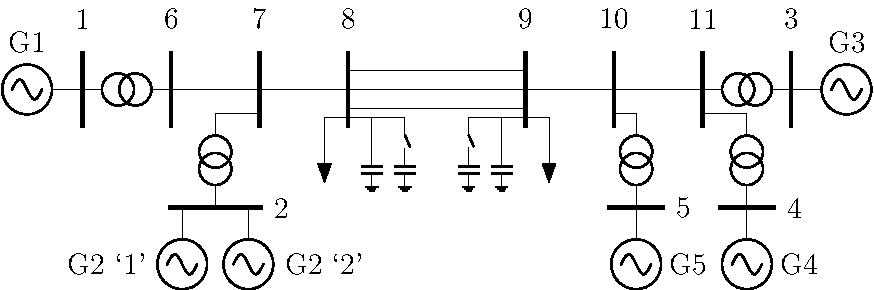
\includegraphics[width=\linewidth]{../../models/sixMachine/sixMachine}
\paragraph{Event Description:} Load step of 75 MW on bus 9 when t=5. \\Area 1 is scheduled to send 100 MW to Area 2 for the entire simulation.
\paragraph{Simulation Agents:}
This simulation uses step, power plant, and balancing authority agents. An example of how such agents are defined in code is shown below.
\begin{lstlisting}[language=Python]
# Perturbances
# Defined as a list of single quote strings.
mirror.sysPerturbances = [
    'load 9 : step P 5 75 rel', # Step Load P +75 MW relative at t=5
    ]

# Power Plants
# Defined as a dictionary of lists of strings
mirror.sysPowerPlants ={'pp1': ["gen 2 1: 0.75 : rampA", "gen 2 2 : 0.25: rampA"],
                        'pp2': ["gen 3 : 0.75: rampA", "gen 4 : 0.25: rampA"],
                        }

# Testing of Balancing Authority input
# Defined as a dictionary of dictionaries
mirror.sysBA = {
    'BA1':{
        'Area':1,
        'B':" 1.0 : p", # MW/0.1 Hz -> 1.0 percent of initial Area load
        'ActionTime': 5.00, # sends update signals as requred every x seconds
        'Type':'TLB : 0', # Tie-Line Bias : conditional ACE parts
        'Filtering': 'PI : 0.1 0.0001', # where 0.1 = Kp, and 0.0001 = a = Ki/Kp
        'CtrlGens': ['plant pp1 : .60 ',
                    'gen 1 : .40 : rampA']
        },
    'BA2':{
        'Area':2,
        'B':" 1.0 : p", # MW/0.1 Hz
        'ActionTime': 5.00,
        'Type':'TLB : 0', # Tie-Line Bias
        'Filtering': 'PI : 0.1 0.0001',
        'CtrlGens': ['plant pp2 : 1.0 ']
        },
    }
\end{lstlisting}

\pagebreak
\paragraph{ACE Definition:} Positive ACE denotes over generation. $B$ (the frequency bias) is negative.
\begin{align*}
\text{ACE}_{\text{tie line}} &= P_{gen} - P_{load} - P_{\text{sched interchange}}\\
\text{ACE}_{\text{frequency bias}} &= 10B(f_{\text{actual}}-f_{\text{sched}})f_{base}\\
\text{ACE} &= \text{ACE}_{\text{tie line}} -\text{ACE}_{\text{frequency bias}}
\end{align*}

\paragraph{Initial Step ACE Results:} Initial tests where calculated ACE was distributed as steps resulted with an undesirable and unrealistic system response.
\newcommand{\caseName}{SixMachineStepBA}
\newcommand{\testNum}{}
\begin{figure}[h!]
		\centering
		\includegraphics[width=\linewidth]{\caseName BA1}\vspace{-1em}
		%\caption{Generator Electrical Power Output}
		%\label{ Pe}		 
\end{figure}\vspace{-1.5em}
\begin{figure}[h!]
		\centering
		\includegraphics[width=\linewidth]{\caseName BA2}\vspace{-1em}
		%\caption{Generator Mechanical Power Output (un-governed machines have no PSDS data)}
		%\label{ Pm}		 
\end{figure}\vspace{-1.5em}
\begin{figure}[h!]
		\centering
		\includegraphics[width=\linewidth]{\caseName ACE}\vspace{-1em}
		%\caption{Reactive Power Output}
		%\label{ Q}		 
\end{figure}\vspace{-1.5em}
\begin{figure}[h!]
		\centering
		\includegraphics[width=\linewidth]{\caseName Freq}\vspace{-1em}
		\caption{Relevant Balancing Authority Simulation Data from Initial Test.}
		\label{stepTest}		 
\end{figure}\vspace{-1.5em}
\pagebreak
\paragraph{Ramp PI ACE Results:} Changing the ACE distribution to ramps and using a PI controller to filter ACE with a proportional gain of 0.1 and integral gain of 10E-6 produces the responses shown in Figure \ref{PI 0 Results}. The filtered, or \emph{smoothed}, ACE (SACE) is distributed to controlled machines according to their participation factor. The 20 minute simulation uses a 1 second time step.
\renewcommand{\testNum}{0}
\begin{figure}[h!]
		\centering
		\includegraphics[width=\linewidth]{\caseName\testNum BA1}\vspace{-1em}
		%\caption{Generator Electrical Power Output}
		%\label{ Pe}		 
\end{figure}\vspace{-1.5em}
\begin{figure}[h!]
		\centering
		\includegraphics[width=\linewidth]{\caseName\testNum BA2}\vspace{-1em}
		%\caption{Generator Mechanical Power Output (un-governed machines have no PSDS data)}
		%\label{ Pm}		 
\end{figure}\vspace{-1.5em}
\begin{figure}[h!]
		\centering
		\includegraphics[width=\linewidth]{\caseName\testNum ACE}\vspace{-1em}
		%\caption{Reactive Power Output}
		%\label{ Q}		 
\end{figure}\vspace{-1.5em}
\begin{figure}[h!]
		\centering
		\includegraphics[width=\linewidth]{\caseName\testNum Freq}\vspace{-1em}
		\caption{Relevant Balancing Authority Simulation Data Using Ramps and PI Filtering.}
		\label{PI 0 Results}		 
\end{figure}\vspace{-1.5em}

\pagebreak
\paragraph{ACE Filtering Results 1:} Using the previous PI controller, logic was added to always act on frequency bias ACE and only dispatch tie line ACE if it is the same sign as frequency deviation ($f_{actual} - f_{sched}$). This causes the system frequency to return to 60 Hz much faster, but also introduces minor frequency oscillations around t=180.
\renewcommand{\testNum}{1}
\begin{figure}[h!]
		\centering
		\includegraphics[width=\linewidth]{\caseName\testNum BA1}\vspace{-1em}
		%\caption{Generator Electrical Power Output}
		%\label{ Pe}		 
\end{figure}\vspace{-1.5em}
\begin{figure}[h!]
		\centering
		\includegraphics[width=\linewidth]{\caseName\testNum BA2}\vspace{-1em}
		%\caption{Generator Mechanical Power Output (un-governed machines have no PSDS data)}
		%\label{ Pm}		 
\end{figure}\vspace{-1.5em}
\begin{figure}[h!]
		\centering
		\includegraphics[width=\linewidth]{\caseName\testNum ACE}\vspace{-1em}
		%\caption{Reactive Power Output}
		%\label{ Q}		 
\end{figure}\vspace{-1.5em}
\begin{figure}[h!]
		\centering
		\includegraphics[width=\linewidth]{\caseName\testNum Freq}\vspace{-1em}
		\caption{Relevant Balancing Authority Simulation Data Using Conditional Distribution.}
		\label{PI 1 Results}		 
\end{figure}\vspace{-1.5em}
\pagebreak


\paragraph{ACE Filtering Results 2:} Expanding on the previous filtering rules, ACE is only distributed when it is the same sign as frequency deviation. In this case, system recovery speed is still improved, frequency oscillations are not present near the steady state, and unnecessary Pref adjustment in Area 1 is eliminated.
\renewcommand{\testNum}{2}
\begin{figure}[h!]
		\centering
		\includegraphics[width=\linewidth]{\caseName\testNum BA1}\vspace{-1em}
		%\caption{Generator Electrical Power Output}
		%\label{ Pe}		 
\end{figure}\vspace{-1.5em}
\begin{figure}[h!]
		\centering
		\includegraphics[width=\linewidth]{\caseName\testNum BA2}\vspace{-1em}
		%\caption{Generator Mechanical Power Output (un-governed machines have no PSDS data)}
		%\label{ Pm}		 
\end{figure}\vspace{-1.5em}
\begin{figure}[h!]
		\centering
		\includegraphics[width=\linewidth]{\caseName\testNum ACE}\vspace{-1em}
		%\caption{Reactive Power Output}
		%\label{ Q}		 
\end{figure}\vspace{-1.5em}
\begin{figure}[h!]
		\centering
		\includegraphics[width=\linewidth]{\caseName\testNum Freq}\vspace{-1em}
		\caption{Relevant Balancing Authority Simulation Data With Refined Conditional Distribution.}
		\label{PI 2 Results}		 
\end{figure}\vspace{-1.5em}

\pagebreak


\paragraph{ACE Filtering Results 3:} Again expanding on the previous filtering rules, proportional controller gain was reduced to 0.02 while the integral gain was set at 2E-6 (80\% reduction in both cases).\\ This allows for a clearer definition between governor and AGC action without the use of deadbands.\vspace{-1.5em}
\renewcommand{\testNum}{3}
\begin{figure}[h!]
		\centering
		\includegraphics[width=\linewidth]{\caseName\testNum BA1}\vspace{-1em}
		%\caption{Generator Electrical Power Output}
		%\label{ Pe}		 
\end{figure}\vspace{-1.5em}
\begin{figure}[h!]
		\centering
		\includegraphics[width=\linewidth]{\caseName\testNum BA2}\vspace{-1em}
		%\caption{Generator Mechanical Power Output (un-governed machines have no PSDS data)}
		%\label{ Pm}		 
\end{figure}\vspace{-1.5em}
\begin{figure}[h!]
		\centering
		\includegraphics[width=\linewidth]{\caseName\testNum ACE}\vspace{-1em}
		%\caption{Reactive Power Output}
		%\label{ Q}		 
\end{figure}\vspace{-1.5em}
\begin{figure}[h!]
		\centering
		\includegraphics[width=\linewidth]{\caseName\testNum Freq}\vspace{-1em}
		\caption{Relevant Balancing Authority Simulation Data with Conditional Distribution and Reduced Control Effort.}
		\label{PI 2 Results}		 
\end{figure}\vspace{-1.5em}

\paragraph{Quasi-Conclusions:} There are many ways to manipulate distribution of ACE to achieve a desired system response. Simulations are a good way to verify system operation. \\

PSLTDSim (the software I've been writing for the past 7-ish months) is a simulation tool that can perform various long-term control experiments involving governors and AGC.
\end{document}